\documentclass[12pt,a4paper]{article}

\usepackage[utf8]{inputenc}
\usepackage[T1]{fontenc}
\usepackage[french]{babel}
\usepackage{fancyhdr}
\usepackage{graphicx}
\usepackage{eurosym}

           

\title{Project llama~~--~ Cahier des Charges}
\date{}

\author{
                Ludovic \textit{Capsir} (allard\_l) \and
                Valentin \textit{Super Nuoc Man} (gramal\_v) \and
                Martin \textit{Nanotek} (zaarou\_m) \and
                Alexis \textit{Sousouil} (anseau\_a) \and
}


\pagestyle{fancyplain} \chead{}\lhead{\textit{Ice Owls}} \rhead{\emph{\textit{Project llama}}}

\begin{document}

\maketitle
\begin{figure}[hp]
          \centering
          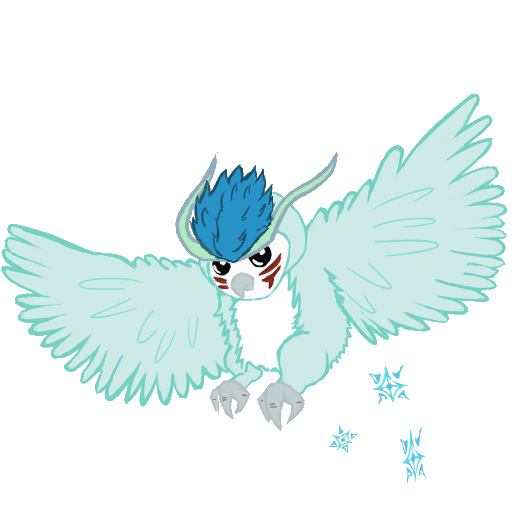
\includegraphics[width=1.00\textwidth]{ice_owl_clear.png}
          
\end{figure}


\newpage
\tableofcontents
\newpage

\section*{Introduction}
\addcontentsline{toc}{section}{Introduction}

Dans le cadre de notre première année d'études à l'EPITA, nous sommes tenus de réaliser un projet dans les six mois qui nous sont impartis. Ce cahier des charges vous présentera les détails les plus intimes de notre projet.\\

Nous nous connaissions déjà avant de rentrer dans cette école et c'est pour cela que nous avons choisis de former ce groupe ensemble. Ainsi, nous sommes convaincus qu'il y aura une bonne entente qui permettra d'arriver au terme de ce projet dans les meilleures conditions.\\

Au programme du jeu, un RPG en 2D. C'est un jeu qui nous permettrait d'aborder différents aspects de la programmation tant ses possibilités sont nombreuses. En effet, ce dernier est très exploité au niveau commercial, il existe de nombreuses licences, une des plus connues étant \textit{The Legend of Zelda}.\\

Nous avons l'espoir de réaliser un jeu fun, qui se distingue des autres et qui procure autant de plaisir que celui mentionné ci-dessus.\\

\newpage
\section{Présentation du groupe}
 
  \subsection{Ludovic \textit{Capsir} }
Jeune homme de 19 ans, fan d'innovation et de high-tech, je suis un bidouilleur dans l'âme. Débutant en programmation mais pressé d'apprendre, j'ai été nommé chef de ce projet. Je prends donc ce dernier très à cœur et espère bien le mener jusqu'au bout contre vents et marrées. Ce jeu a une ambition, le fun, pour moi le premier but d'un jeu est de détendre. Mon expérience de gamer n'ai pas très grande mais mes camarades sont la pour combler ma faiblesse. Have Fun


  \subsection{Valentin \textit{Super Nuoc Man}}

Bonjour bonjour, moi c'est Valentin alias Super Nuoc Man. J'ai depuis très longtemps été geek,  surtout dans les jeux vidéo, c'est pourquoi j'ai toujours voulu en créer un. J'ai donc toucher à de nombreux types de gameplay et je pourrais avoir de bons conseils à donner à mon groupe pour celui de notre jeu.
Mes bases en programmation sont presque nulles mais je compte bien apprendre efficacement tout au long de l'année pour venir a bout de notre projet.
Je sais que mes compagnons n'ont pas une très grande culture WTF de l'internet c'est pourquoi je suis la pour apporter quelques références de qualité qui donneront de l‘originalité au projet.
Je suis fan de manga et d'animation japonaise et j'ai un certain sens artistique que les autres membre du groupe Ice Owls n'ont pas c'est pourquoi je m'occupe de toute la partie graphique du projet.
Les lamas domineront le monde !

  \subsection{Martin \textit{Nanotek}}
Joueur depuis toujours, le jeu vidéo est mon hobbie préféré. Fan de la série Kingdom Hearts, sortie sur PS2, j'aimerais faire un jeu agréable, malgré le fait que nous soyons les Ice Owls et non Square Enix . J'aime les mangas , malgré le peu de mangas différents que je lis. Je suis un dresseur de pokemon, venant du Bourg Palette. Lorsque je suis allé cherché mon Pokemon chez le professeur Chen , les trois pokemons étaient déjà pris , ce qui me força à prendre Pikachu comme pokemon. J'ai entrepris d'être le meilleur dresseur, que je me battrais sans répit, je ferais tout pour être le vainqueur, et gagner les défis. Je parcourrais la Terre entière, me battant avec espoir .

  \subsection{Alexis \textit{Sousouil}}

Bonjour moi c'est Alexis aka Sousouil, passionné par les jeux vidéos depuis toujours (no-life à certaines périodes), avoir la chance d'en créer un est une belle opportunité à saisir. N'ayant jamais codé auparavant je ne désire pas être non plus trop ambitieux pour ce projet là, même si j'espère une bonne entraide dans le groupe qui me permettra un progrès rapide en programmation.
Je suis aussi un hyper-actif qui à toujours besoin de bouger et toujours son mot à dire, en espérant que cela permette une bonne dynamique au sein du groupe.

\newpage

\section{Le Projet}
      \subsection{Un RPG}
Un RPG est un jeu de rôle où le joueur incarne un personnage principal qui évolue dans un environnement constitué de plusieurs maps et d'autres personnages. Le personnage est libre de se déplacer a travers cette environnement mais cependant est guidé tout au long du jeu par une quête principale. Le héros gagnera en expérience et en caractéristique au cours de son histoire.\\

Il sera possible d'interagir avec les autres personnages, permettant de faire avancer le joueur à travers différents dialogues et quêtes secondaires.

\begin{figure}[hp]
          \centering
          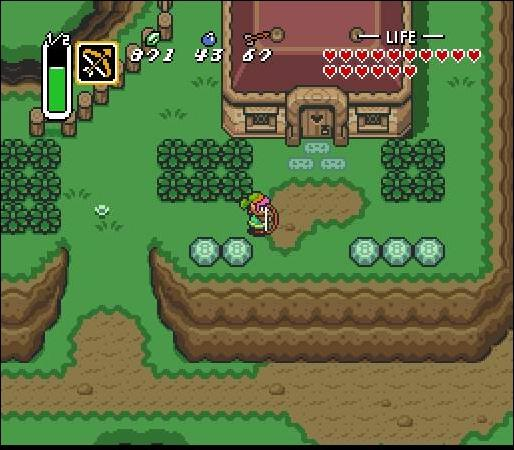
\includegraphics[scale=0.60]{image-zelda.jpg}
\caption{Legend of Zelda}
\label{fig:}
          
\end{figure}
\newpage

\subsection{Thème}
Le jeu se déroulera entre deux mondes. Dans le premier, le héros se déplacera dans une ambiance médiévale avec des châteaux et villages, le second monde sera celui où le héros évoluera durant ses missions, l'environnent sera alors futuriste et minimal à la manière de Tron. Le passage entre les deux mondes se feras via les donjons qui seront comme des portails de téléportations

      \subsection{A Faire }

\subsubsection{Graphismes}

Nous avons choisi de faire un jeu en 2D pour plusieurs raisons. D'une part nous voulons faire des graphismes du style pixel-art ce qui permettra un meilleur rendu. De plus, le joueur pourra avoir une vision globale de la map.
L'ensemble des graphismes ( textures, niveaux ,menus,...) sera dessiné par nos soins rendant ainsi notre jeu unique. 
Enfin un moteur graphique sera créé pour afficher l'ensemble du jeu.

\subsubsection{Moteur Physique}

Le moteur physique nous sera utile pour tout ce qui est collisions, déplacements de personnages ou délimitations des cartes et sera donc un des plus gros point de notre projet sur lequel on devra se concentrer. En effet, un RPG n'est rien sans un moteur physique digne de ce nom (traverser un arbre ou une maison n'est pas commun à tout le monde). Par exemple, le moteur physique devra prendre en compte l'interaction du personnage avec tout son environnement comme les arbres, les objets sur le sol, etc.
Le moteur physique nous permettra ainsi d'avoir un jeu dont le gameplay sera satisfaisant.

\subsubsection{Intelligence Artificielle}

L'intelligence artificielle dans le jeu permettra d'avoir des monstres pas trop ridicules qui agiront en fonction de l'emplacement du joueur et des attaques qu'ils disposeront ainsi qu'en fonction du statut du héros ou des actions qu'il effectuera. Par exemple, si l'on s'approche trop près d'un monstre, qu'on se trouve dans son champs de vision, alors il se déplacera automatiquement vers nous.\\


\subsubsection{Audio}

Comme dans beaucoup de jeux qui marquent, tel que\textit{ The Legend of Zelda}, nous essayerons d'avoir des musiques s'adaptant à toutes les situations ce qui mettra le joueur dans de bonnes conditions de jeu. Ainsi, cela créera une ambiance dans le quel le joueur pourra s'immerger.

\subsubsection{Multijoueur}

Pour le multijoueur, nous créerons un mode coopération dans lequel deux joueurs, sur le même ordinateur, devront s'entraider pour terminer à bien leur mission. Une expérience supplémentaire sera donc ajouter pour donner plus de fun au gameplay.

\subsubsection{Site Web}

Le site web: http://www.project-llama.fr nous permettra d'informer sur l'avancement du projet pour les personnes intéressées qu'elles soient francophone ou anglophone. L'ensemble des sources des documents du projet y seront disponible en téléchargement. De plus d'un point de vue marketing nous mettrons à disposition des "goodies", c'est-à-dire des fonds d'écran, des t-shirts, des mugs, ou autres objets de la sorte.


\newpage

\section{Organisation}

     
      \subsection{Planning}
            \subsubsection{Première soutenance}
 \begin{tabular}{|l|c|c|c|c|c|c|}
            \hline
                             & Graphisme & Moteur Physique & IA & Audio & Multi & Site Web \\ \hline
            Ludovic        &   30~\%   & &   & 25~\%& &  40~\% \\ \hline
            Alexis           &       &  20~\%   &   10~\% &  &    &  40~\%   \\ \hline
            Valentin        &   30~\%     &   &10~\%  & &   0~\%  &             \\ \hline
           Martin           &      &        20~\%    & &  25~\%  &0~\%  &    \\ \hline
            
        \end{tabular}

            \subsubsection{Deuxième soutenance}

 \begin{tabular}{|l|c|c|c|c|c|c|}
            \hline
                                  & Graphisme & Moteur Physique & IA & Audio & Multi & Site Web \\ \hline
            Ludovic        &   50~\%   & &   & 60~\%& &  100~\% \\ \hline
            Alexis           &       &  50~\%   &   40~\% & &    &  100~\%   \\ \hline
            Valentin        &   50~\%     &   &40~\%  &&   0~\%  &             \\ \hline
           Martin           &      &        50~\%    & &  60~\%  &0~\%  &    \\ \hline
            
        \end{tabular}

            \subsubsection{Troisième soutenance}
 \begin{tabular}{|l|c|c|c|c|c|c|}
            \hline
                                                          & Graphisme & Moteur Physique & IA & Audio & Multi & Site Web \\ \hline
            Ludovic        &   95~\%   & &   & 90~\%& &  100~\% \\ \hline
            Alexis           &       &  75~\%   &   50~\% &  &    &  100~\%   \\ \hline
            Valentin        &  95~\%     &   &50~\%  & &   50~\%  &             \\ \hline
           Martin           &      &        75~\%    & &  90~\%  &50~\%  &    \\ \hline
            
        \end{tabular}

            \subsubsection{Soutenance finale}

 \begin{tabular}{|l|c|c|c|c|c|c|}
            \hline
                           & Graphisme & Moteur Physique & IA & Audio & Multi & Site Web \\ \hline
            Ludovic        &   100~\%   & &   & 100~\%& &  100~\% \\ \hline
            Alexis           &       &  100~\%   &   100~\% &  &    &  100~\%   \\ \hline
            Valentin        &  100~\%     &   &100~\%  &&   100~\%  &             \\ \hline
           Martin           &      &        100~\%    & &  100~\%  &100~\%  &    \\ \hline
        \end{tabular}
\newpage

      \subsection{Moyens et coûts}

Pour ce projet nous utiliserons essetiellement nos ordinateurs personnels ainsi que les nos racks.
Pour la partie logiciel , nous utiliserons 
\begin{itemize}
\item Visual Studio 2010 ultimate (developement)
\item Audacity  (son) 
\item Git (versionnement)
\item The Gimp , Paint tool SAI , Ms Paint (graphisme)
\item Adobe After effect CS5 (graphisme)
\end{itemize}
 
Les logiciels utilisés sont tous disponible gratuitement sur le net ou via Epita, ceci n'engendre donc pas de cout supplémentaire.
\\
\\
\\

\begin{figure}[h!]\begin{center}
\begin{tabular}{|l|l|}
\hline
Type &Montant du devis \\ \hline
Logiciels & 0~\euro{} \\ \hline
T-Shirts du groupe & 100~\euro{} \\ \hline
Nom de domaine , Hebergement & 15~\euro{} \\ \hline
Publicité & 741~\euro{} \\ \hline
Stock d'Ice Tea, Dr Pepper & 1337~\euro{} \\ \hline
5 Fruits \& Légume par jour & 984~\euro{} \\ \hline
\textbf{Total TTC} & Erreur \\ \hline


\end{tabular}
\caption{Budget}
\end{center}\end{figure}


\newpage

\section*{Conclusion}   
Notre projet, vous l'aurez compris, est plutôt ambitieux. Malgré un choix de facilité via des graphismes en 2D, nous avons une réelle envie de faire un jeu complet. Possédant un mode solo avec une IA et un mode multijoueur, notre jeux sera un véritable produit fini. Nous allons également acquérir de nouvelles compétences que ce soit au niveau du travail en groupe, ou de la programmation. Nous espérons que celui-ci vous plaira et vous surprendra.
\\
\\



 Cordialement, l'équipe \textit{Ice Owls}.
\addcontentsline{toc}{section}{Conclusion}



\end{document}
